\chapter{Appendix}
\label{cha:appendix}

\section{Data Exploration}
\label{sec:DataExploration}

% \begin{figure}[H]
%     \centering
%     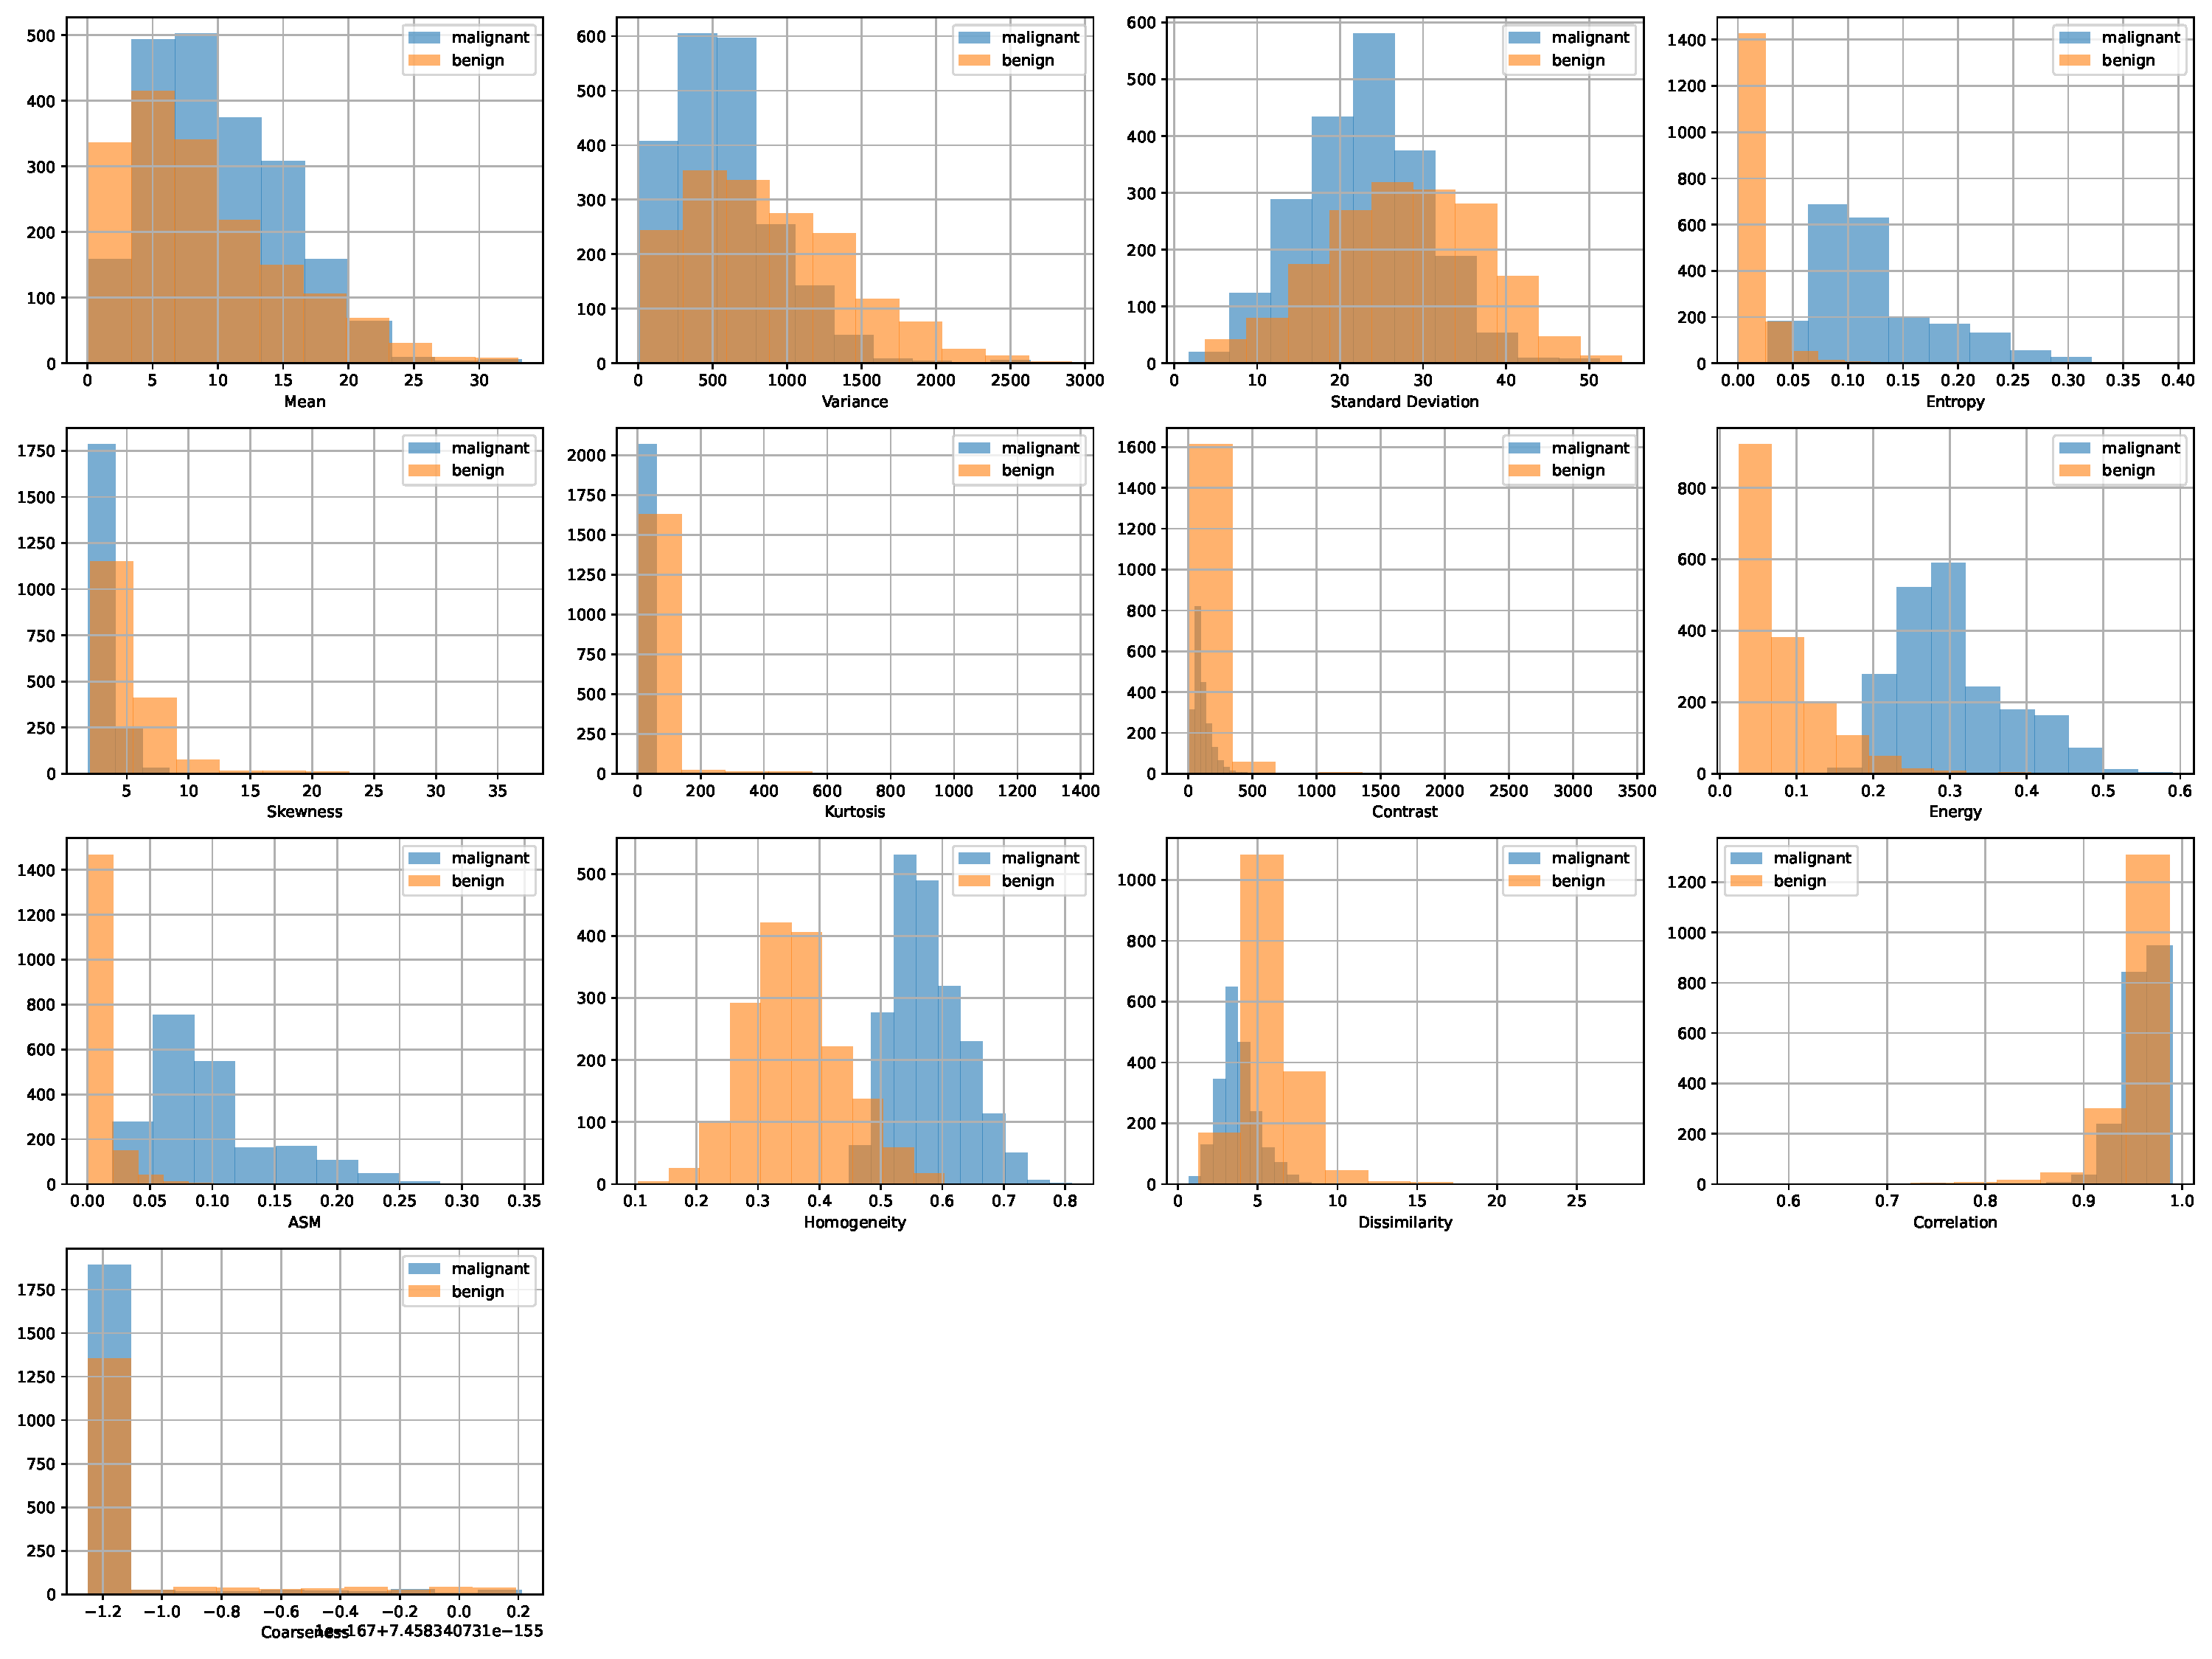
\includegraphics[width=.8\textwidth]{plots/benign_malignant_comparison.pdf}
%     \caption{Comparison between benign and malignant brain tumours for the first- and second-order features.}
%     \label{fig:benign_malignant_comparison}
% \end{figure}

The correlation and scatter matrix of the first- and second-order features are shown in figures \ref{fig:correlation} and \ref{fig:scatter_matrix} respectively.
The correlation matrix reflects that the energy, the homogeneity, the entropy and the ASM are highly correlated with the class and are as such the most promising features to distinguish between benign and malignant brain tumours.

\begin{figure}
    \centering
    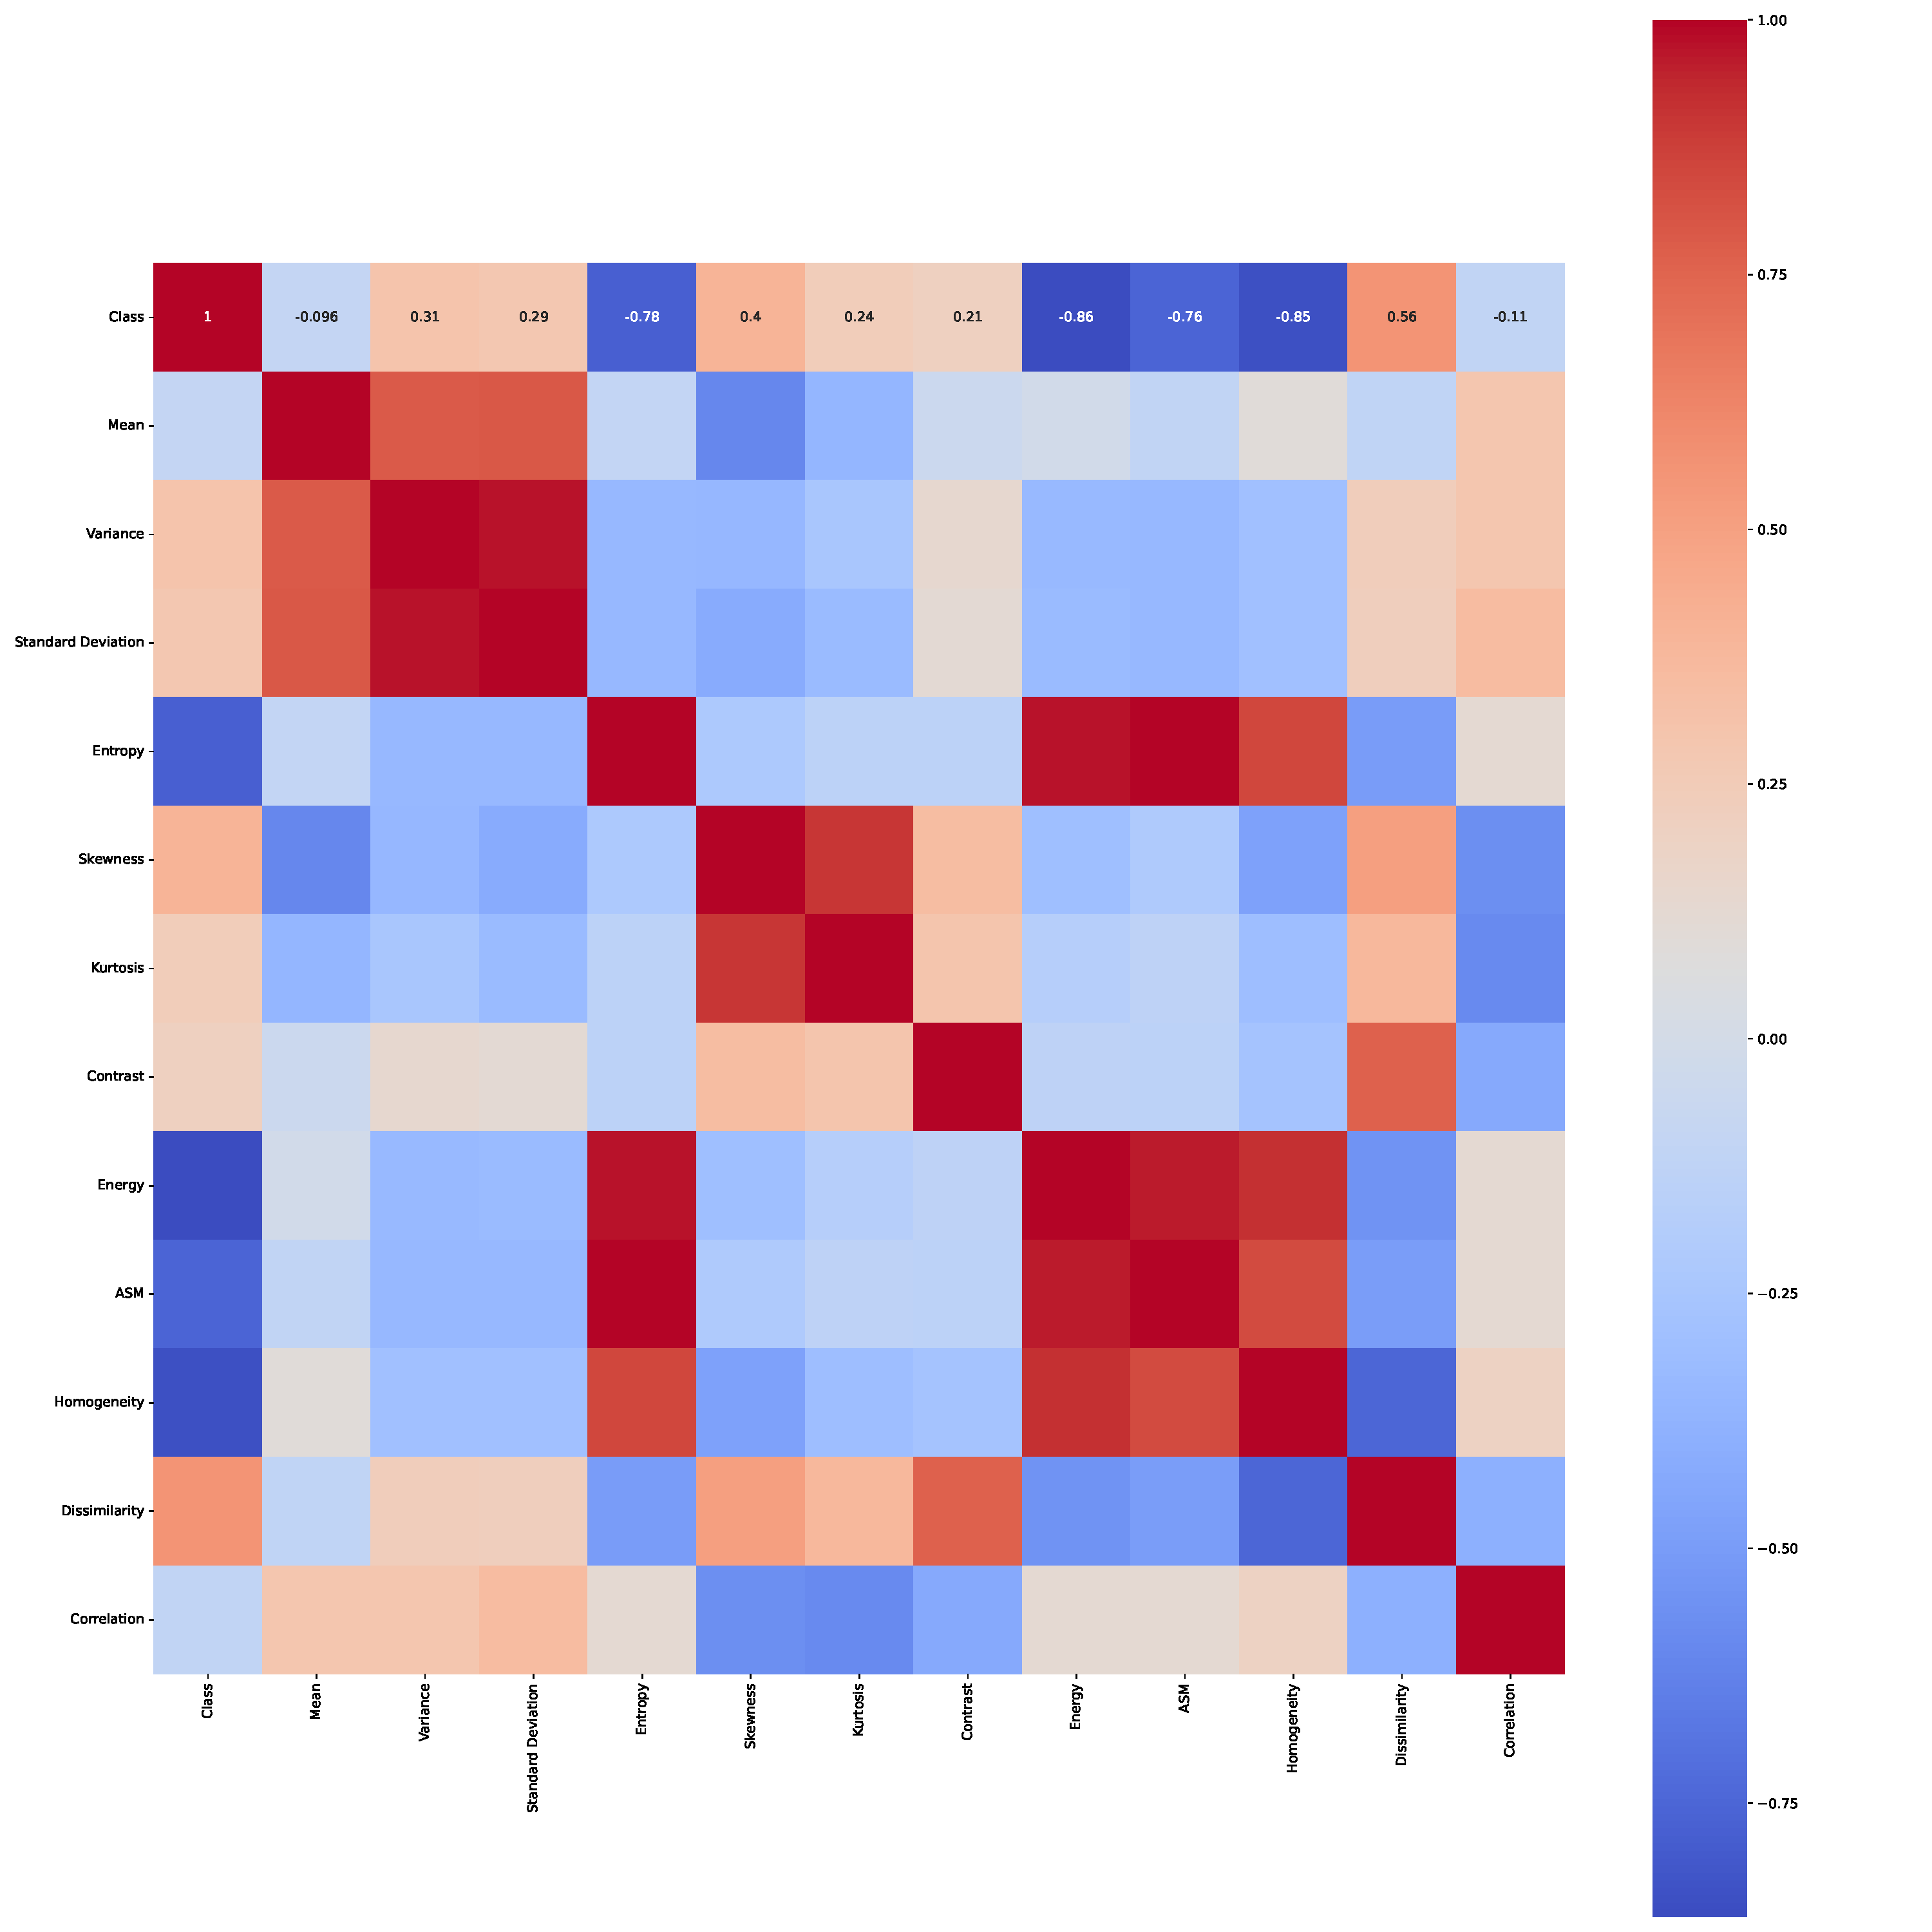
\includegraphics[width=1.2\textwidth]{plots/correlation.pdf}
    \caption{Correlation of the first- and second-order features.}
    \label{fig:correlation}
\end{figure}

\begin{figure}
    \centering
    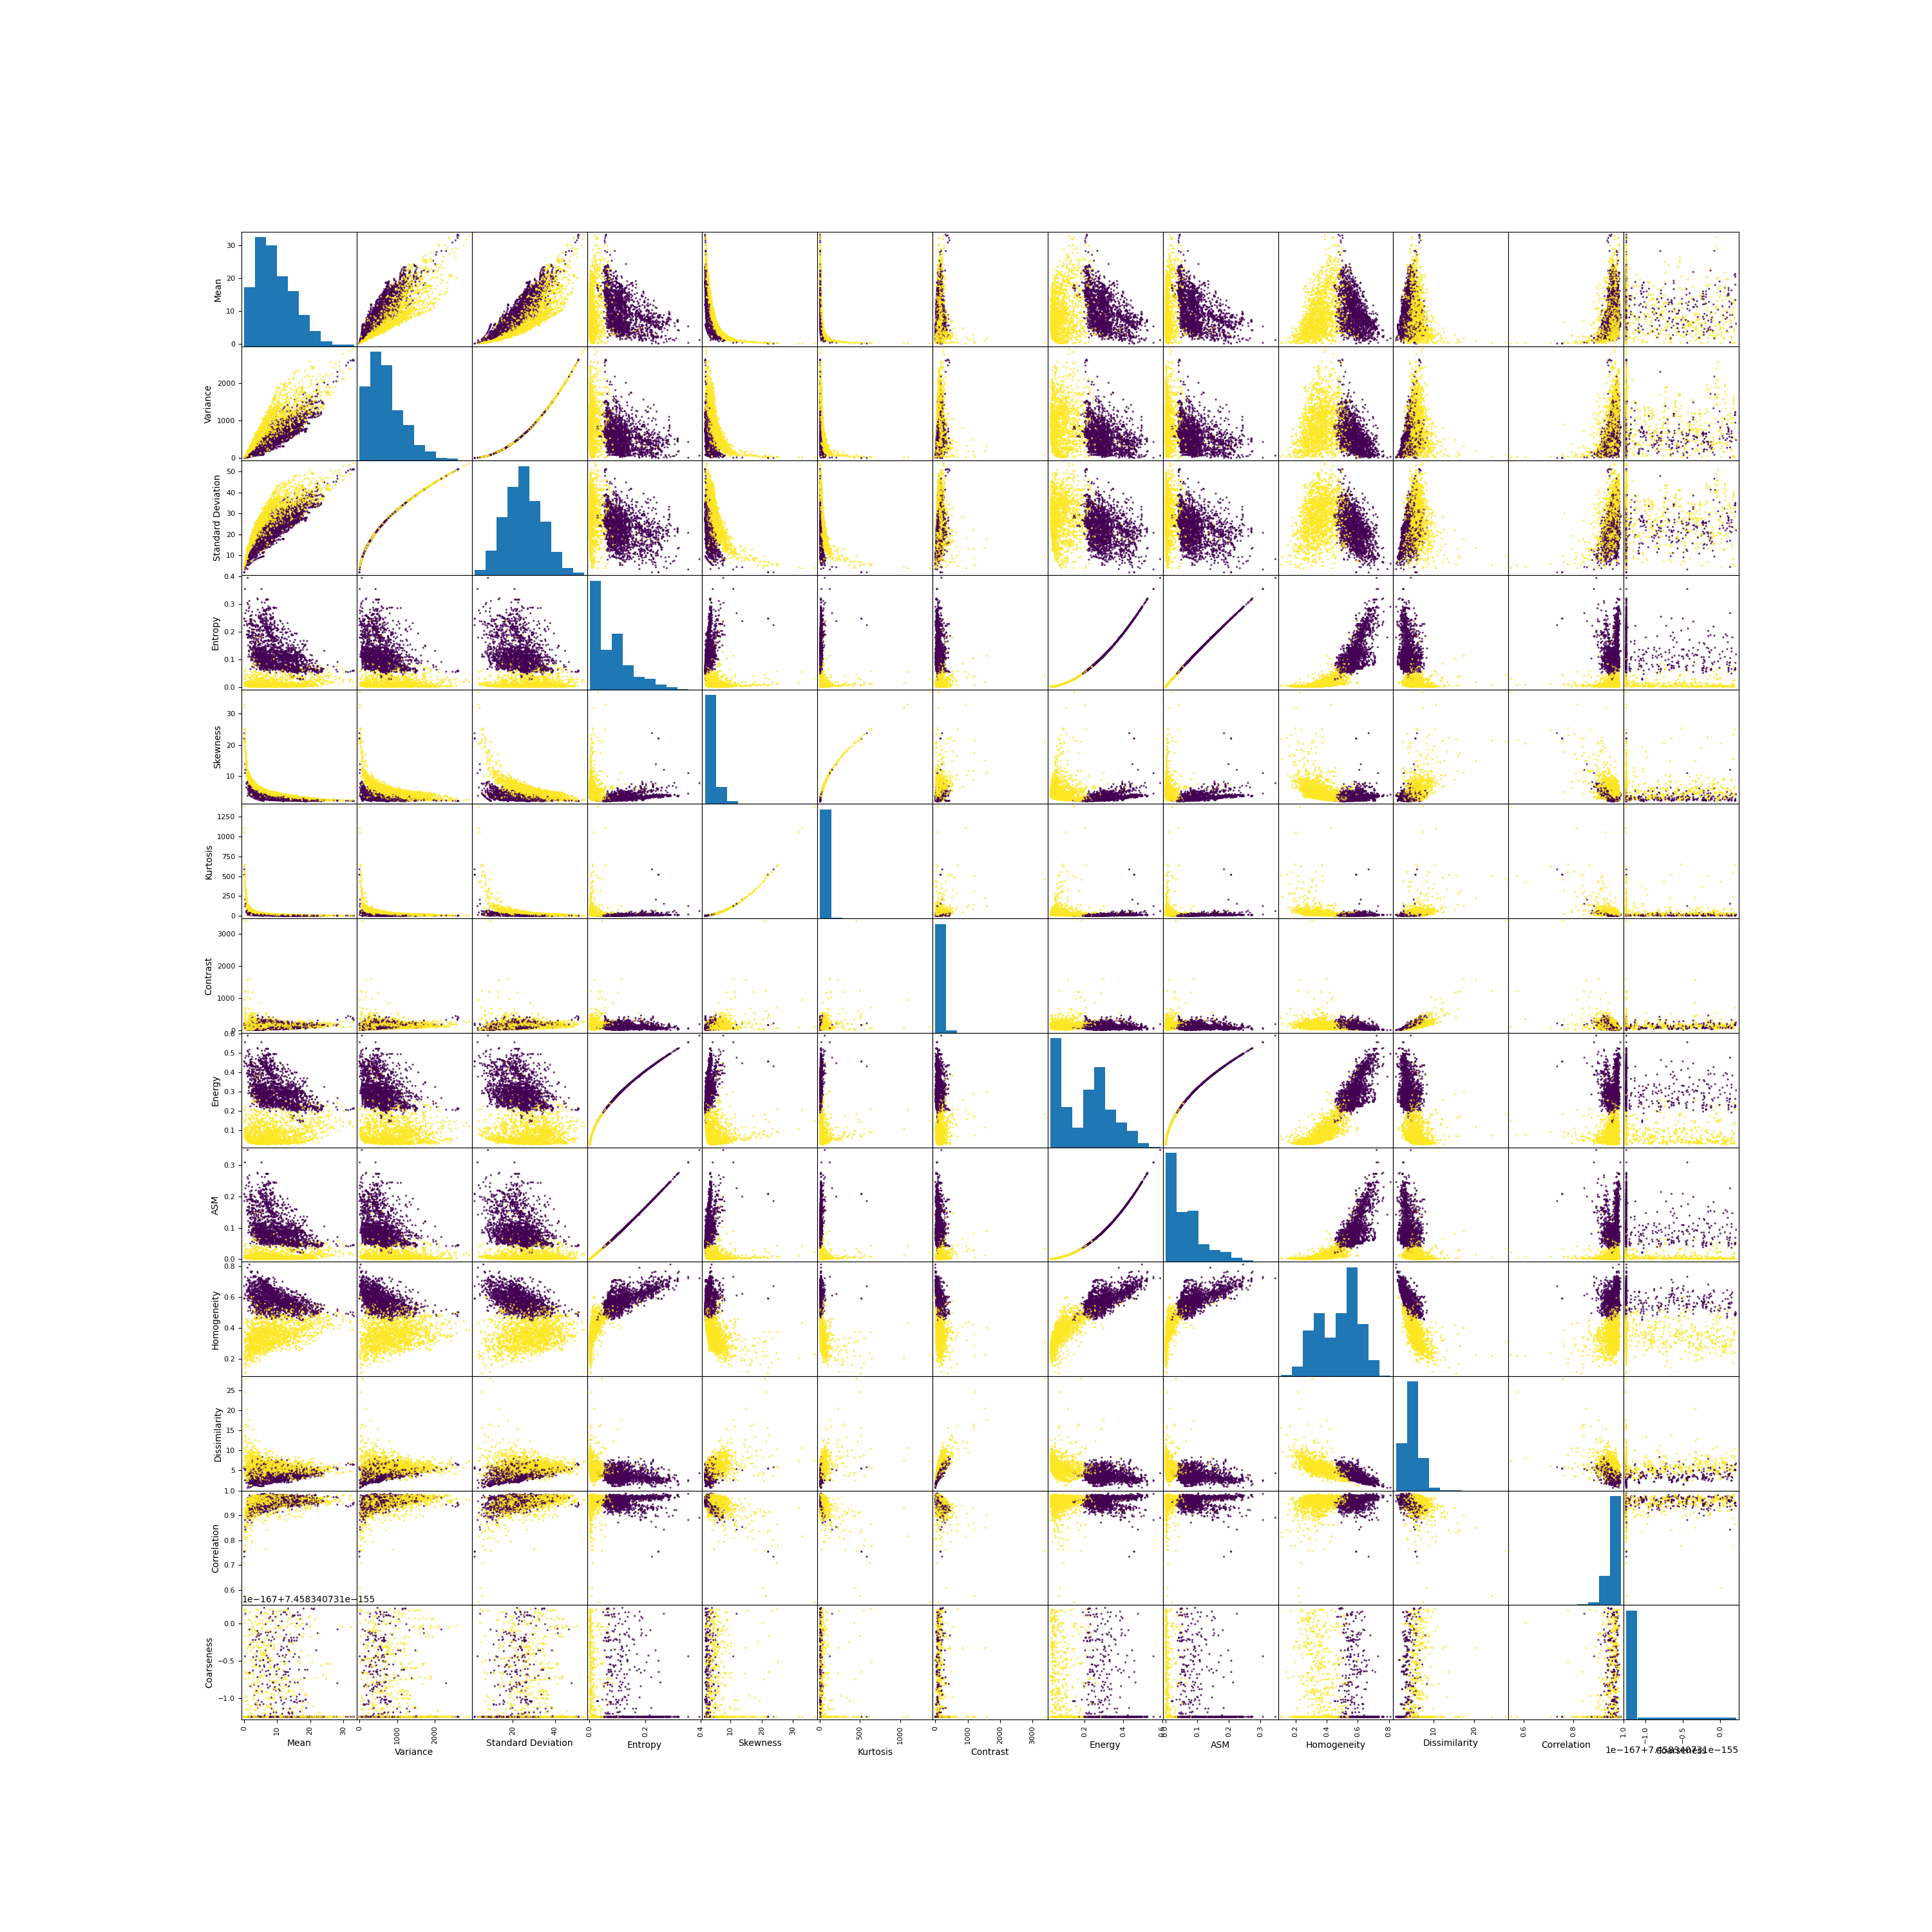
\includegraphics[width=1.2\textwidth]{plots/scatter_matrix.png}
    \caption{Scatter matrix of the first- and second-order features.}
    \label{fig:scatter_matrix}
\end{figure}


\section{First Gridsearch Hyperparameter Tests}
\label{sec:FirstGridsearchHyperparameterTests}

Figure \ref{fig:FirstHyperparameterTests} shows the first hyperparameter tests using gridsearch.
This hyperparameter test led to the test, which is described in section \ref{sec:hyperparameter}.
The main goal was to reduce the overfitting, which is why the delta between the training and validation loss was used as the main metric. 
Because the dropout rate decreased the delta between the training and validation loss so much, it was decided to increase the dropout range to 0.6 in the next test.
Because the number of dense units did not have an impact on the delta, a higher range was chosen for the next test.
The range of the number of filters in the convolutional layers was not increased as the delta increased with the number of filters.
There was only taken more data for the next test by using more filters in the same range.

\begin{figure}[H]
    \centering
    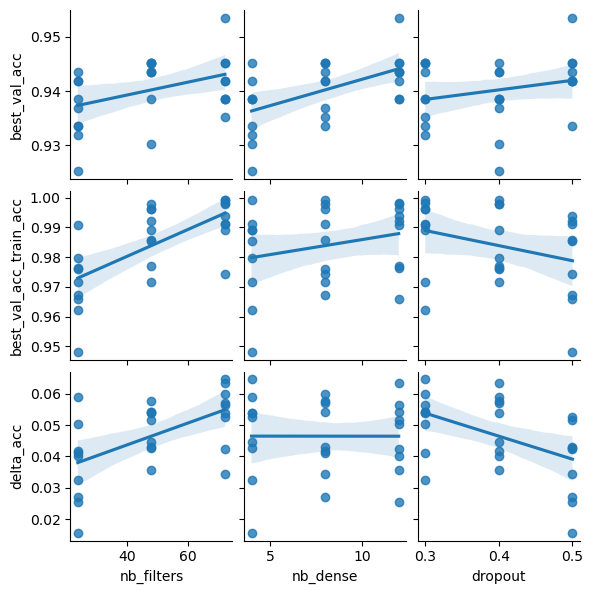
\includegraphics[width=.8\textwidth]{plots/FirstHyperparameterTests.png}
    \caption{First hyperparameter tests using gridsearch.}
    \label{fig:FirstHyperparameterTests}
\end{figure}

% \section{Code}
% \label{sec:Code}

% The code can be found in the corresponding GitHub repository \cite{project} or directly via the \href{https://github.com/joeyko2706/MachineLearning24/tree/main}{link}.
% Alternatively, you may find the code below.
% \includepdf[pages={1-}]{./content/Project.pdf}